\subsection{Experimental Results}\label{sec:release_results}
The preliminary results use the free-polarized baseline described above. Only statistical errors are shown, including the propagated dilution uncertainty for the target-dependent ratios. Point-to-point selection, background, nuclear, radiative and polarization-scale uncertainties have not been assigned to these plots. The $LU$ result retains six $-t'$ bins per $x_B$ interval, while both $UL$ ratios use three. Individual points compatible with zero are retained. The $LL$ amplitudes float in the fits but are not included in the conference release.
The beam-spin ratio shows a resolved change of sign with $-t'$ in the lowest $x_B$ interval. The value near $\langle-t'\rangle=0.54$~GeV$^2$ is $-0.1045\pm0.0213$, whereas the first bin is positive. At the highest $x_B$ the six values remain positive, approximately $0.08$--$0.10$. The intermediate intervals retain additional structure that would be lost by integrating over $-t'$.
The three-bin $UL\sin\phi$ results resolve forward negative values in the two middle $x_B$ intervals: $-0.1174\pm0.0368$ and $-0.0912\pm0.0323$. Several higher-$-t'$ points are less precise. The $UL\sin2\phi$ measurements provide constraints with varying precision. The positive higher-$-t'$ values, including $0.4950\pm0.2285$ in $0.35<x_B<0.45$, are retained as measured points without treating them as established signals. Results compatible with zero remain part of the release.

\begin{table}[htbp]\centering
\begin{tabular}{lrr}\toprule
Sample & Selected combinations & Unique events\\\midrule
RGB\_spring2019\_D2 & 544,503 & 542,668\\
RGB\_fall2019\_D2 & 200,768 & 199,874\\
RGB\_spring2020\_D2 & 253,382 & 252,480\\
RGC\_summer2022\_ND3 & 62,830 & 62,496\\
RGC\_fall2022\_ND3 & 121,849 & 121,184\\
RGC\_spring2023\_ND3 & 43,318 & 43,153\\
\bottomrule\end{tabular}
\caption{Selected physics samples after the relaxed processing and offline selection.}\label{tab:release_counts}
\end{table}

\begin{figure}[p]\centering
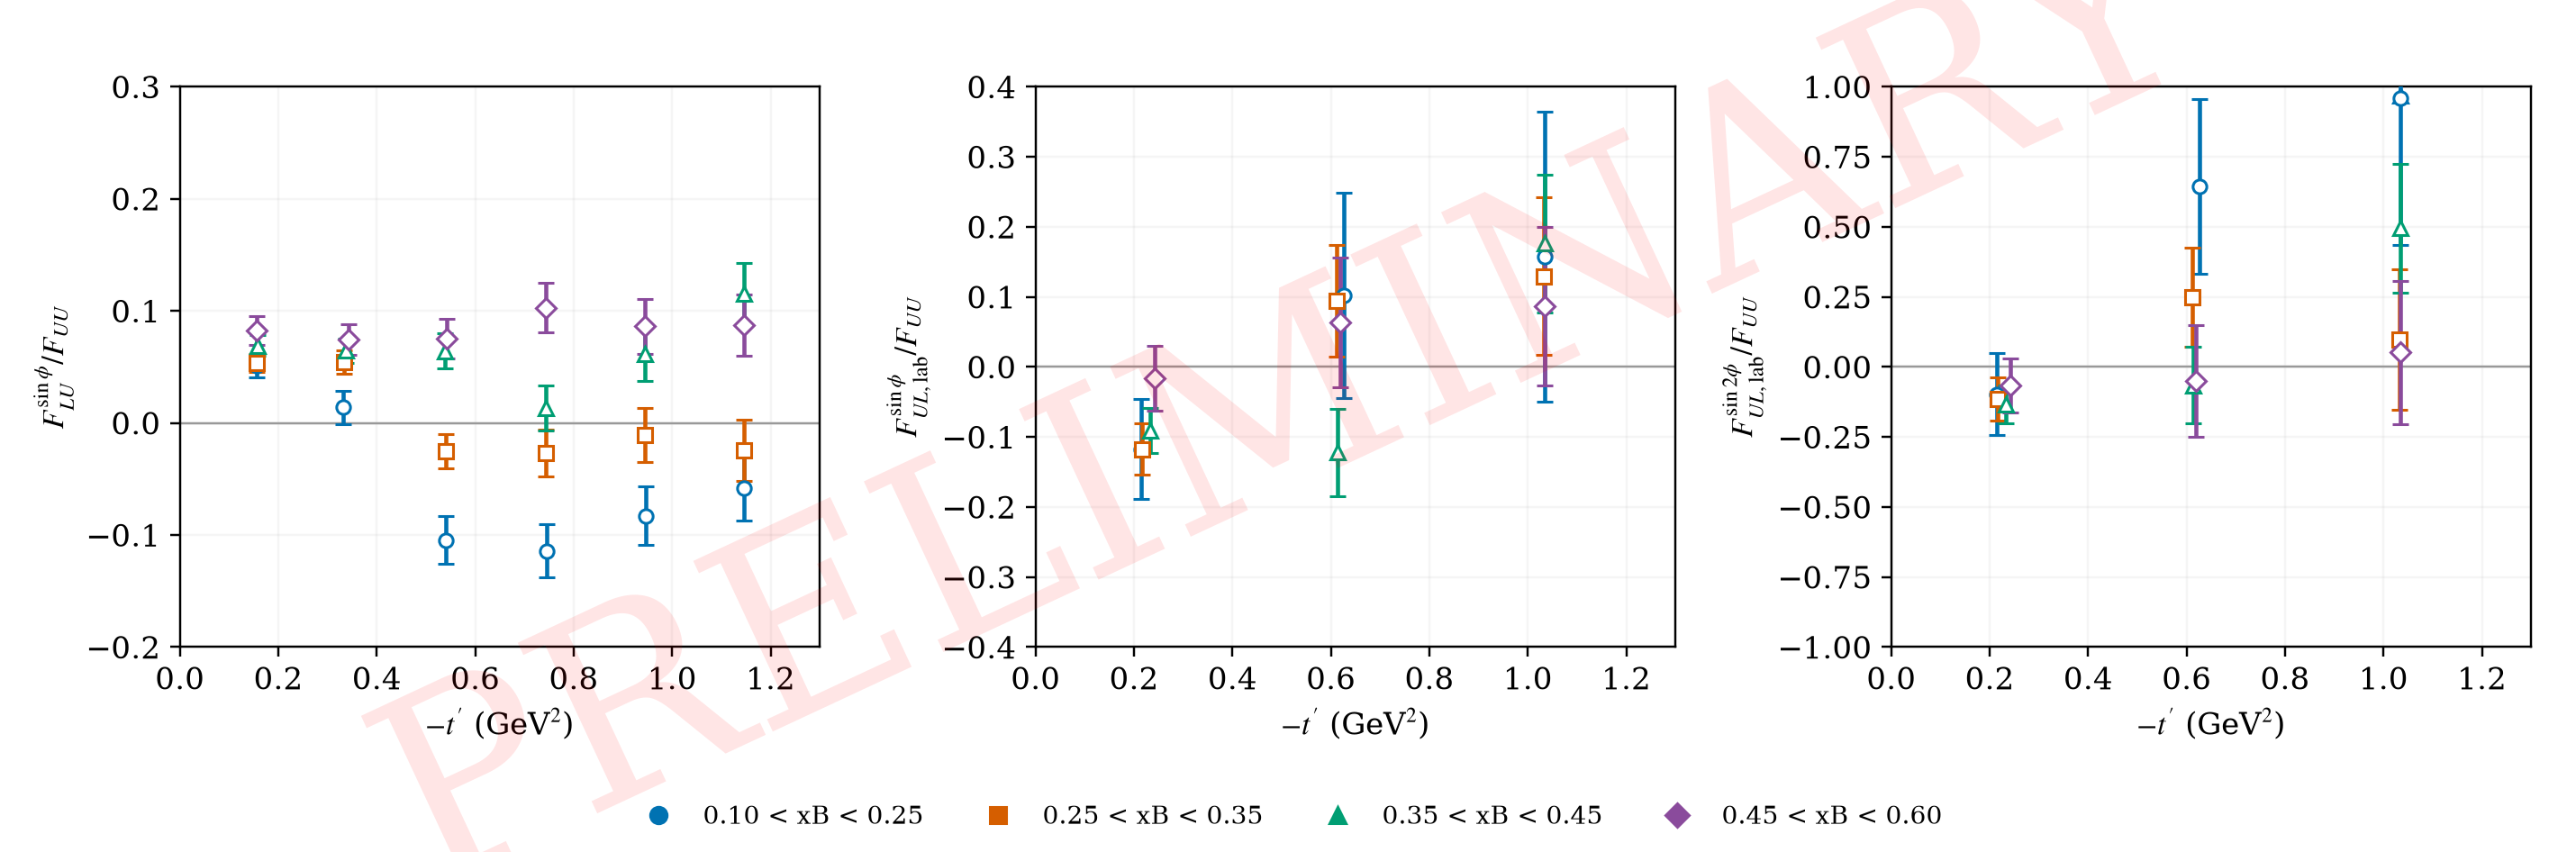
\includegraphics[width=\linewidth]{figures/results/data_overlay_all_xB.png}
\caption{Preliminary $LU$, $UL\sin\phi$ and $UL\sin2\phi$ ratios. Colors distinguish the four $x_B$ intervals. Error bars are statistical.}\label{fig:release_overlay}
\end{figure}
\clearpage
\begin{figure}[p]\centering
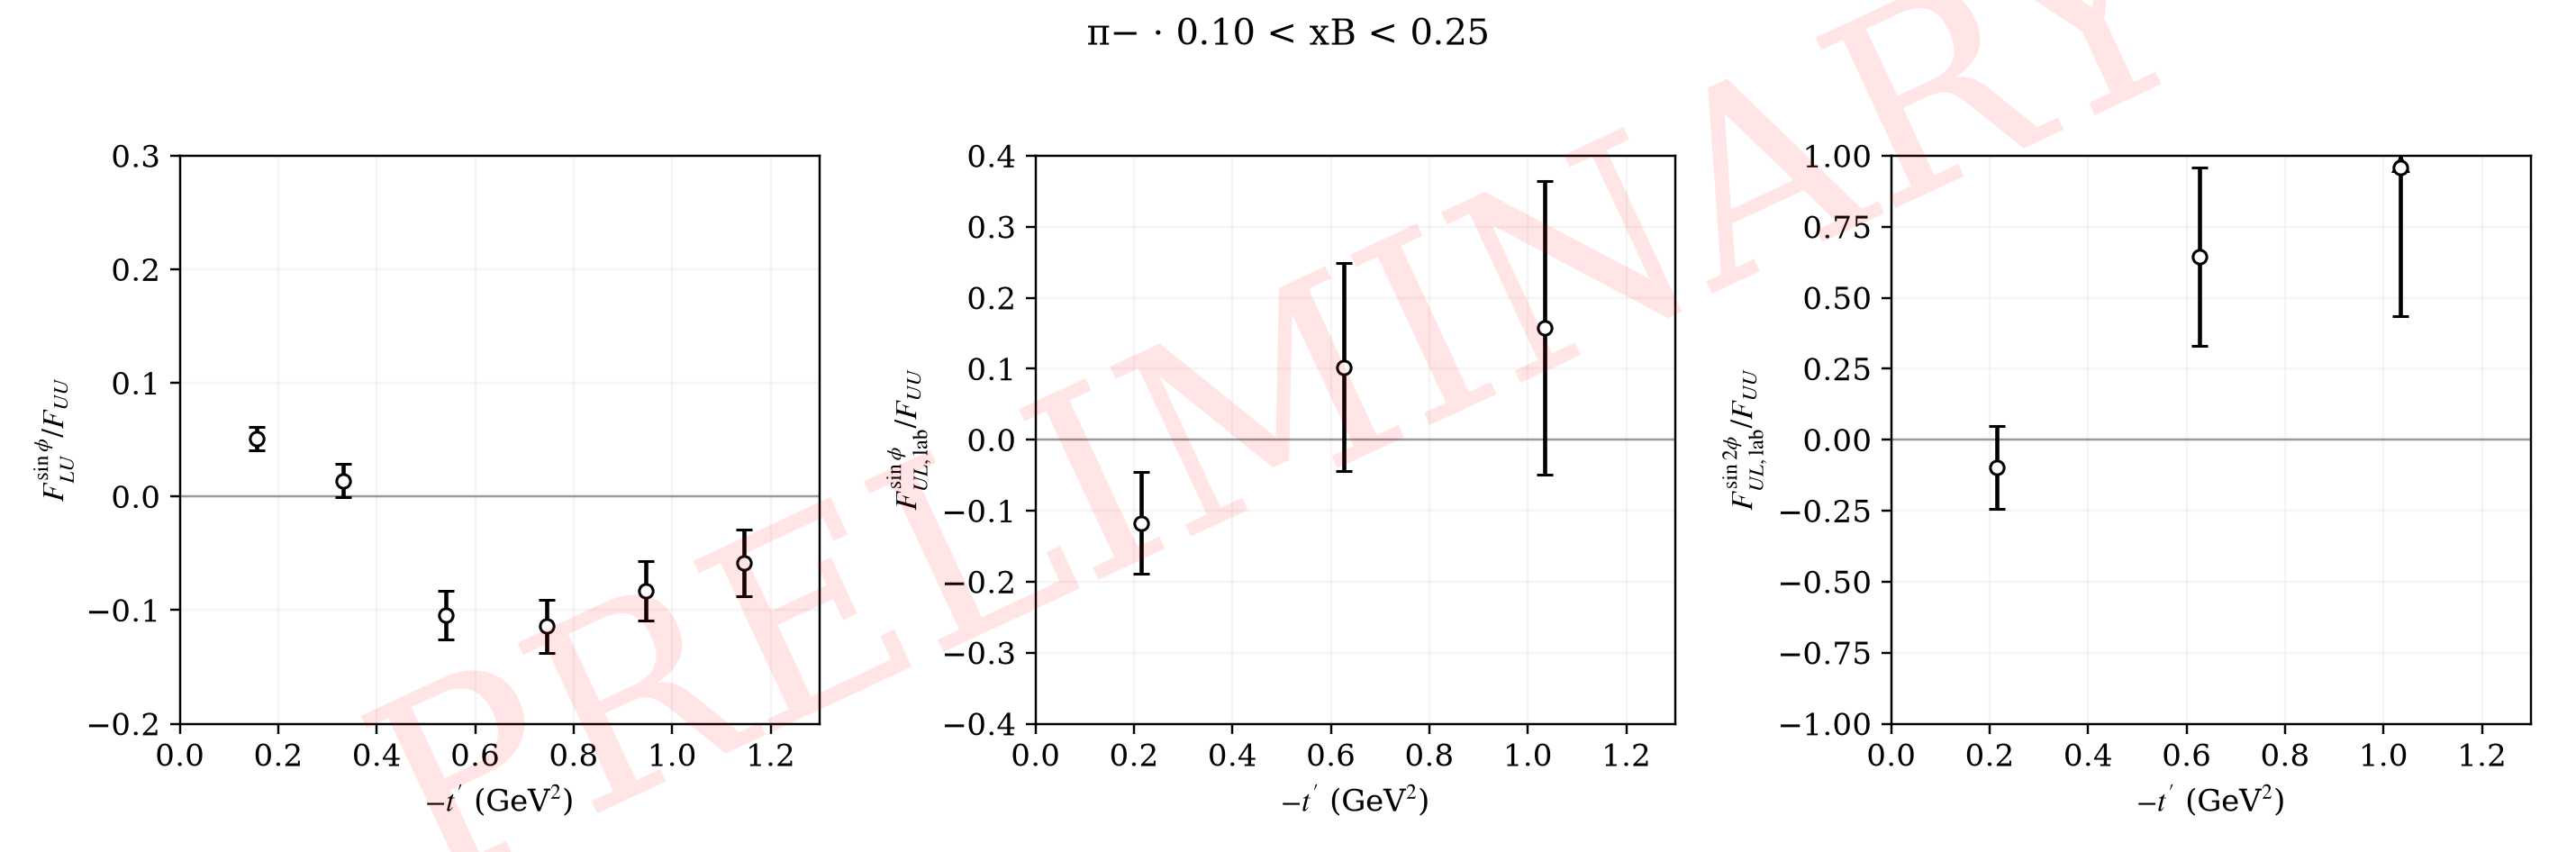
\includegraphics[width=\linewidth]{figures/results/data_xB_bin_1.png}
\caption{Preliminary spin-dependent ratios in $x_B$ interval 1. The $LU$ panel has six $-t^\prime$ bins and each $UL$ panel has three.}\label{fig:release_xb1}
\end{figure}
\clearpage
\begin{figure}[p]\centering
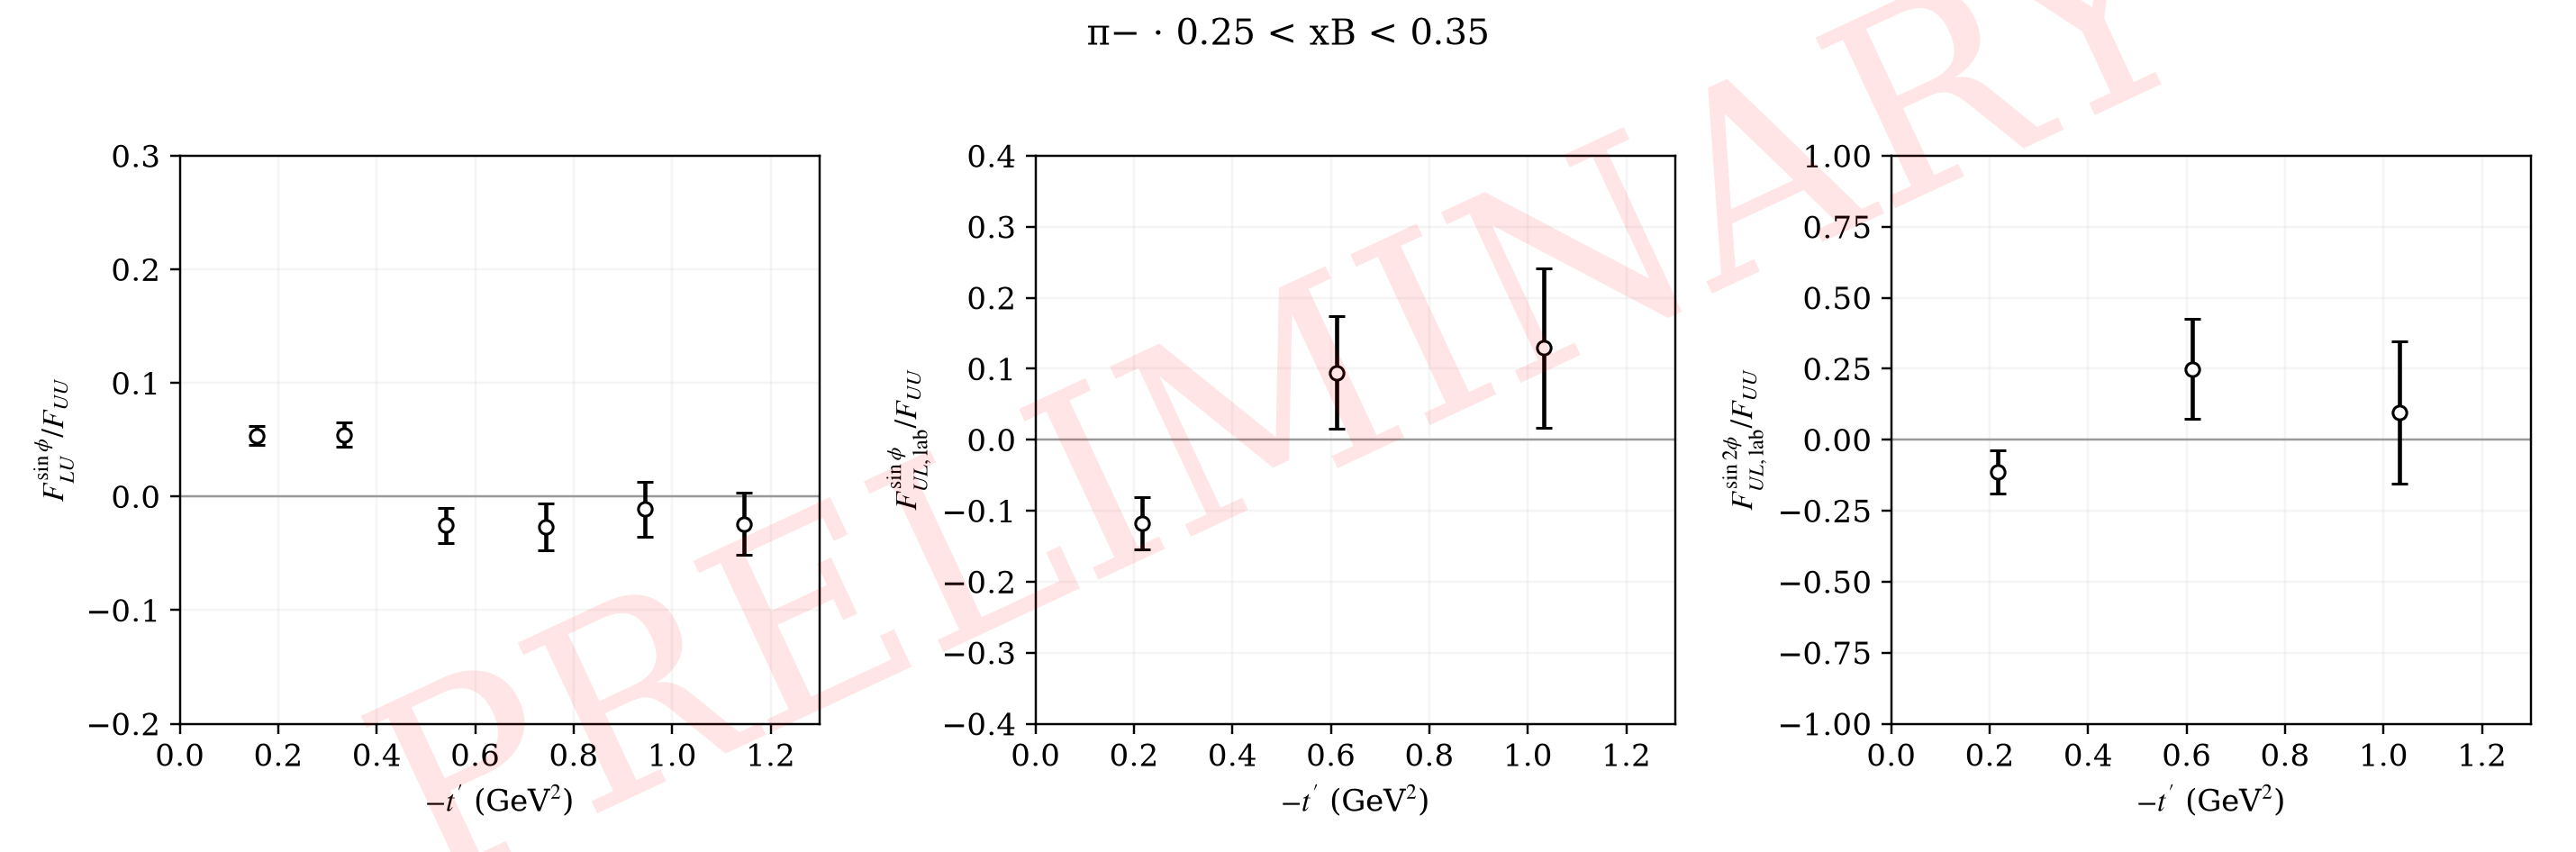
\includegraphics[width=\linewidth]{figures/results/data_xB_bin_2.png}
\caption{Preliminary spin-dependent ratios in $x_B$ interval 2. The $LU$ panel has six $-t^\prime$ bins and each $UL$ panel has three.}\label{fig:release_xb2}
\end{figure}
\clearpage
\begin{figure}[p]\centering
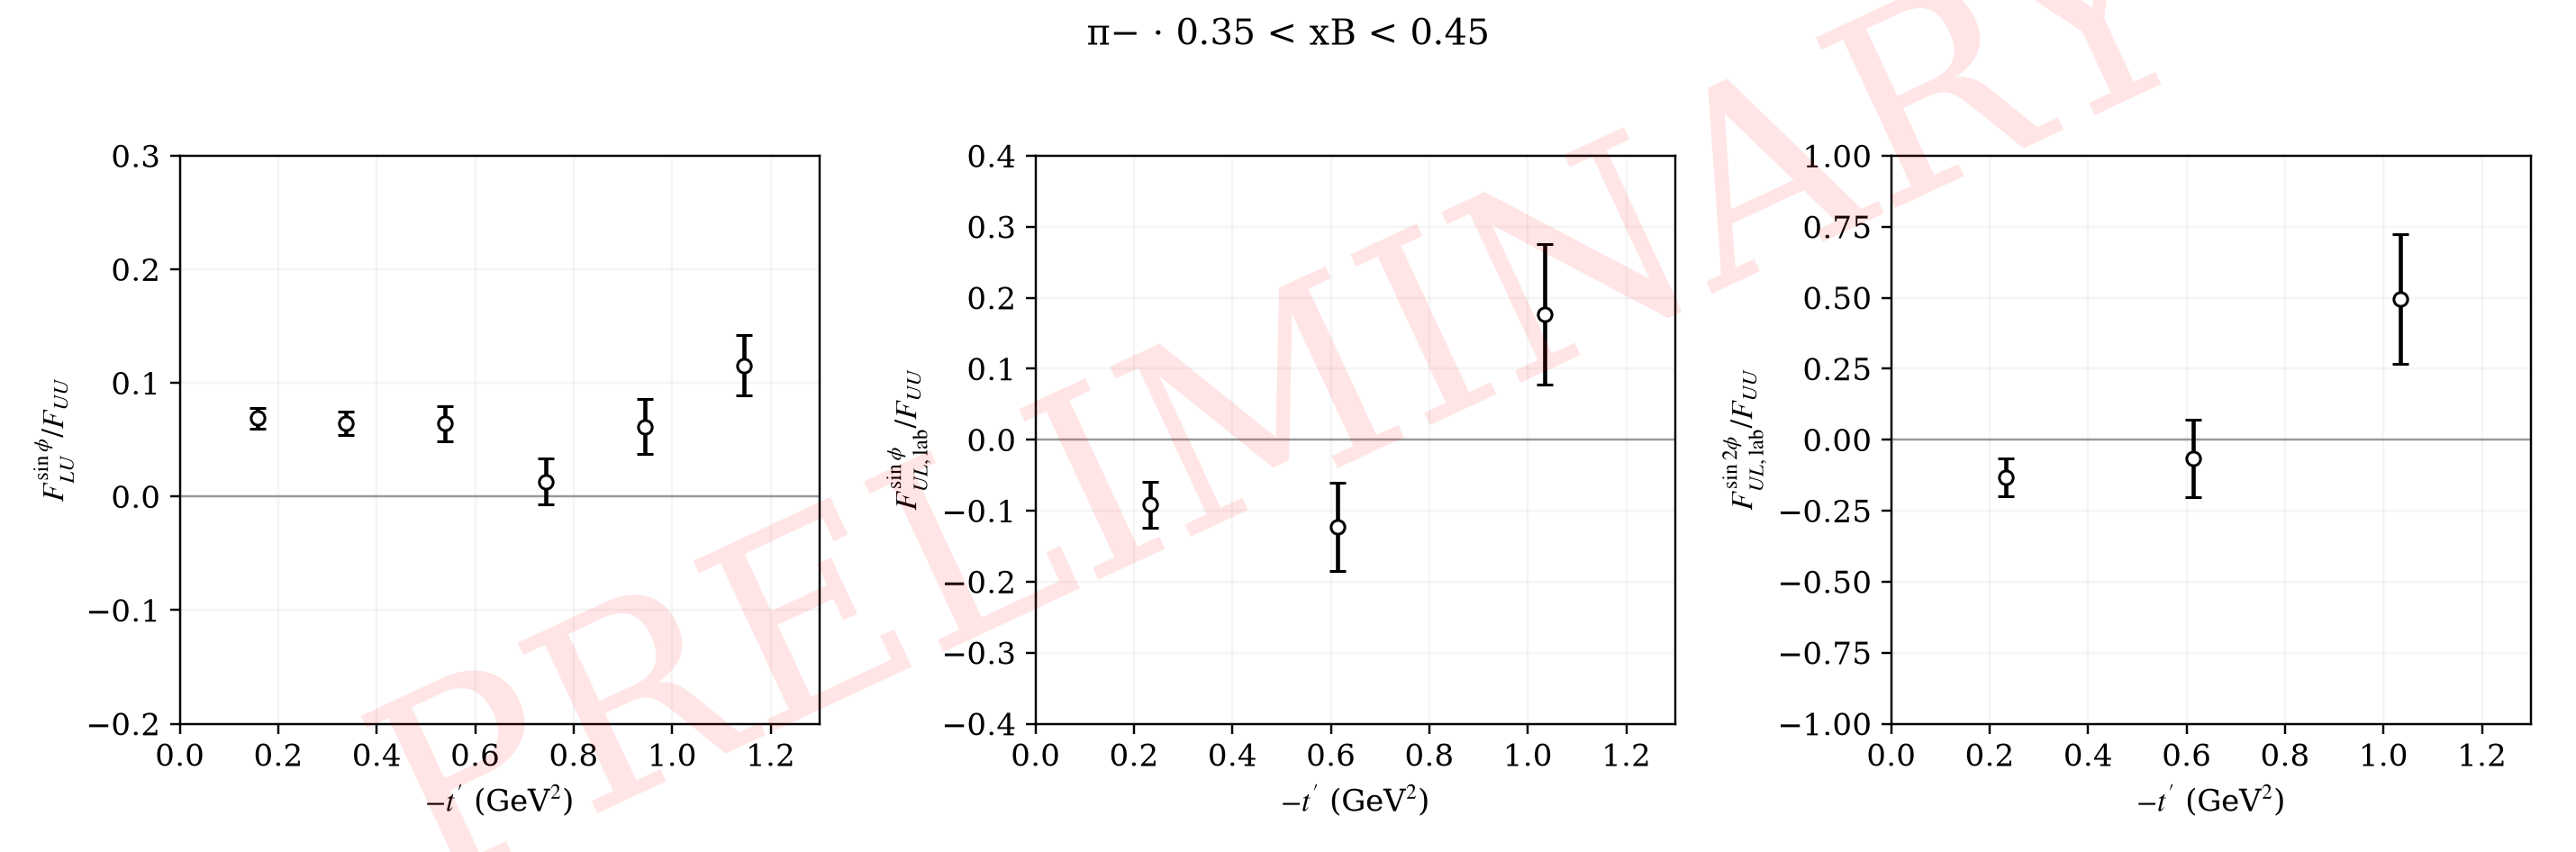
\includegraphics[width=\linewidth]{figures/results/data_xB_bin_3.png}
\caption{Preliminary spin-dependent ratios in $x_B$ interval 3. The $LU$ panel has six $-t^\prime$ bins and each $UL$ panel has three.}\label{fig:release_xb3}
\end{figure}
\clearpage
\begin{figure}[p]\centering
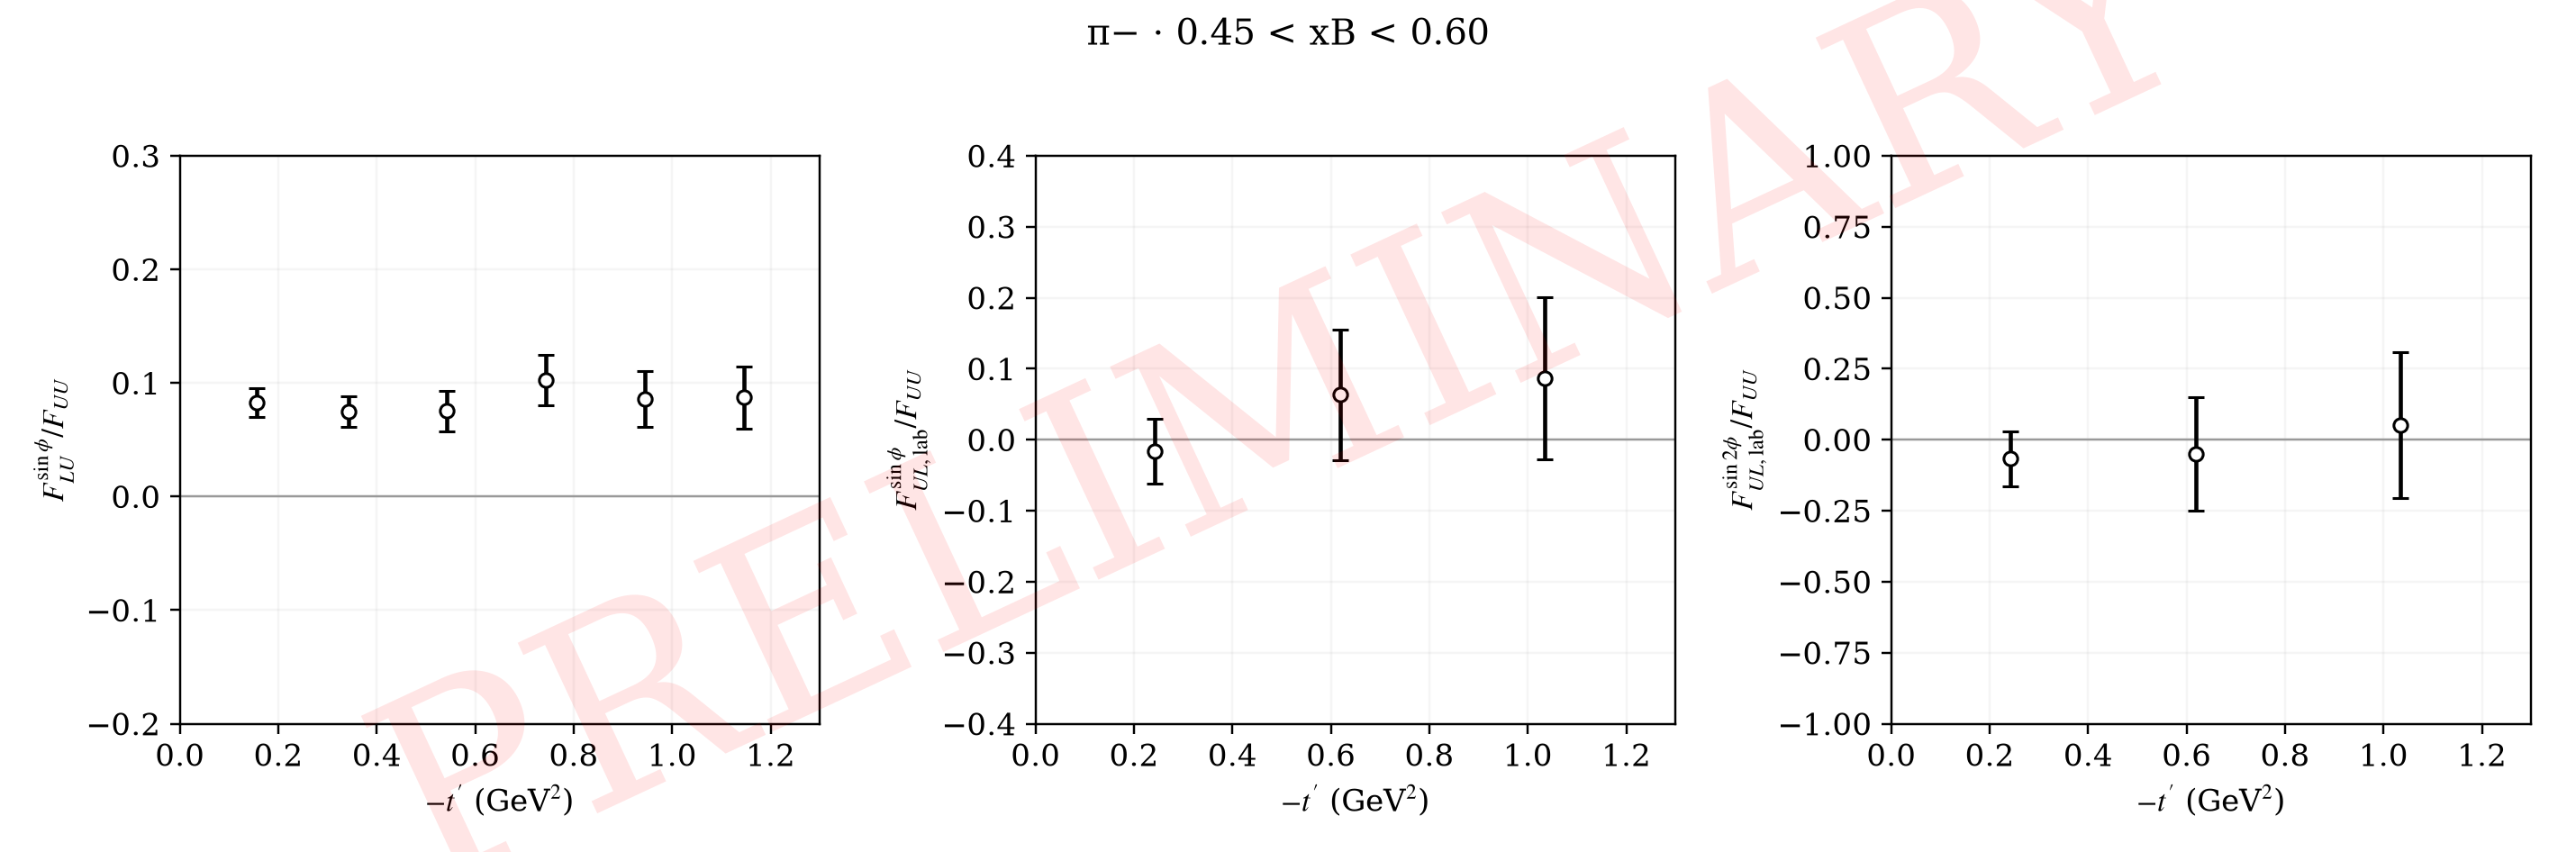
\includegraphics[width=\linewidth]{figures/results/data_xB_bin_4.png}
\caption{Preliminary spin-dependent ratios in $x_B$ interval 4. The $LU$ panel has six $-t^\prime$ bins and each $UL$ panel has three.}\label{fig:release_xb4}
\end{figure}
\clearpage

\clearpage
\begin{longtable}{rrrrr}
\caption{$F_{LU}^{\sin\phi}/F_{UU}$. Statistical uncertainties include dilution propagation where applicable.}\label{tab:release_lu1}\\
\toprule
$x_B$ interval & $-t^\prime$ interval & $\langle-t^\prime\rangle$ & Ratio & Statistical error\\
\midrule\endfirsthead
\toprule $x_B$ interval & $-t^\prime$ interval & $\langle-t^\prime\rangle$ & Ratio & Statistical error\\\midrule\endhead
0.10--0.25 & 0.05--0.25 & 0.156 & 0.0510 & 0.0100\\
0.10--0.25 & 0.25--0.45 & 0.332 & 0.0139 & 0.0146\\
0.10--0.25 & 0.45--0.65 & 0.541 & -0.1045 & 0.0213\\
0.10--0.25 & 0.65--0.85 & 0.745 & -0.1142 & 0.0236\\
0.10--0.25 & 0.85--1.05 & 0.947 & -0.0828 & 0.0260\\
0.10--0.25 & 1.05--1.25 & 1.146 & -0.0582 & 0.0292\\
0.25--0.35 & 0.05--0.25 & 0.157 & 0.0538 & 0.0080\\
0.25--0.35 & 0.25--0.45 & 0.333 & 0.0546 & 0.0105\\
0.25--0.35 & 0.45--0.65 & 0.540 & -0.0253 & 0.0155\\
0.25--0.35 & 0.65--0.85 & 0.743 & -0.0267 & 0.0208\\
0.25--0.35 & 0.85--1.05 & 0.945 & -0.0110 & 0.0241\\
0.25--0.35 & 1.05--1.25 & 1.146 & -0.0241 & 0.0273\\
0.35--0.45 & 0.05--0.25 & 0.158 & 0.0691 & 0.0090\\
0.35--0.45 & 0.25--0.45 & 0.338 & 0.0644 & 0.0106\\
0.35--0.45 & 0.45--0.65 & 0.539 & 0.0641 & 0.0156\\
0.35--0.45 & 0.65--0.85 & 0.743 & 0.0133 & 0.0201\\
0.35--0.45 & 0.85--1.05 & 0.945 & 0.0617 & 0.0244\\
0.35--0.45 & 1.05--1.25 & 1.146 & 0.1156 & 0.0268\\
0.45--0.60 & 0.05--0.25 & 0.156 & 0.0825 & 0.0126\\
0.45--0.60 & 0.25--0.45 & 0.343 & 0.0745 & 0.0135\\
0.45--0.60 & 0.45--0.65 & 0.543 & 0.0754 & 0.0178\\
0.45--0.60 & 0.65--0.85 & 0.744 & 0.1028 & 0.0222\\
0.45--0.60 & 0.85--1.05 & 0.946 & 0.0861 & 0.0246\\
0.45--0.60 & 1.05--1.25 & 1.146 & 0.0874 & 0.0274\\
\bottomrule
\end{longtable}


\clearpage
\begin{longtable}{rrrrr}
\caption{$F_{UL,\mathrm{lab}}^{\sin\phi}/F_{UU}$. Statistical uncertainties include dilution propagation where applicable.}\label{tab:release_ul1}\\
\toprule
$x_B$ interval & $-t^\prime$ interval & $\langle-t^\prime\rangle$ & Ratio & Statistical error\\
\midrule\endfirsthead
\toprule $x_B$ interval & $-t^\prime$ interval & $\langle-t^\prime\rangle$ & Ratio & Statistical error\\\midrule\endhead
0.10--0.25 & 0.05--0.45 & 0.214 & -0.1174 & 0.0715\\
0.10--0.25 & 0.45--0.85 & 0.626 & 0.1023 & 0.1462\\
0.10--0.25 & 0.85--1.25 & 1.034 & 0.1576 & 0.2070\\
0.25--0.35 & 0.05--0.45 & 0.216 & -0.1174 & 0.0368\\
0.25--0.35 & 0.45--0.85 & 0.611 & 0.0947 & 0.0795\\
0.25--0.35 & 0.85--1.25 & 1.032 & 0.1294 & 0.1125\\
0.35--0.45 & 0.05--0.45 & 0.232 & -0.0912 & 0.0323\\
0.35--0.45 & 0.45--0.85 & 0.613 & -0.1221 & 0.0621\\
0.35--0.45 & 0.85--1.25 & 1.034 & 0.1765 & 0.0986\\
0.45--0.60 & 0.05--0.45 & 0.241 & -0.0160 & 0.0460\\
0.45--0.60 & 0.45--0.85 & 0.618 & 0.0636 & 0.0921\\
0.45--0.60 & 0.85--1.25 & 1.034 & 0.0867 & 0.1137\\
\bottomrule
\end{longtable}


\clearpage
\begin{longtable}{rrrrr}
\caption{$F_{UL,\mathrm{lab}}^{\sin2\phi}/F_{UU}$. Statistical uncertainties include dilution propagation where applicable.}\label{tab:release_ul2}\\
\toprule
$x_B$ interval & $-t^\prime$ interval & $\langle-t^\prime\rangle$ & Ratio & Statistical error\\
\midrule\endfirsthead
\toprule $x_B$ interval & $-t^\prime$ interval & $\langle-t^\prime\rangle$ & Ratio & Statistical error\\\midrule\endhead
0.10--0.25 & 0.05--0.45 & 0.214 & -0.0969 & 0.1465\\
0.10--0.25 & 0.45--0.85 & 0.626 & 0.6444 & 0.3133\\
0.10--0.25 & 0.85--1.25 & 1.034 & 0.9739 & 0.5240\\
0.25--0.35 & 0.05--0.45 & 0.216 & -0.1139 & 0.0762\\
0.25--0.35 & 0.45--0.85 & 0.611 & 0.2498 & 0.1774\\
0.25--0.35 & 0.85--1.25 & 1.032 & 0.0965 & 0.2509\\
0.35--0.45 & 0.05--0.45 & 0.232 & -0.1327 & 0.0672\\
0.35--0.45 & 0.45--0.85 & 0.613 & -0.0648 & 0.1360\\
0.35--0.45 & 0.85--1.25 & 1.034 & 0.4950 & 0.2285\\
0.45--0.60 & 0.05--0.45 & 0.241 & -0.0666 & 0.0976\\
0.45--0.60 & 0.45--0.85 & 0.618 & -0.0501 & 0.1992\\
0.45--0.60 & 0.85--1.25 & 1.034 & 0.0513 & 0.2567\\
\bottomrule
\end{longtable}

The period comparisons retain separate likelihood normalizations and the common dilution convention. They are diagnostic comparisons of samples with different within-bin kinematic populations. Across the tested BM-fixed scenarios, the largest changes in $UL\sin\phi$ and $UL\sin2\phi$ are 0.071 and 0.047 times the free-fit statistical error, respectively. The errors themselves are essentially unchanged. These are paired-fit sensitivity scales, not significances. The free baseline is therefore retained without a model constraint on $LL\cos\phi$.
\begin{figure}[p]\centering
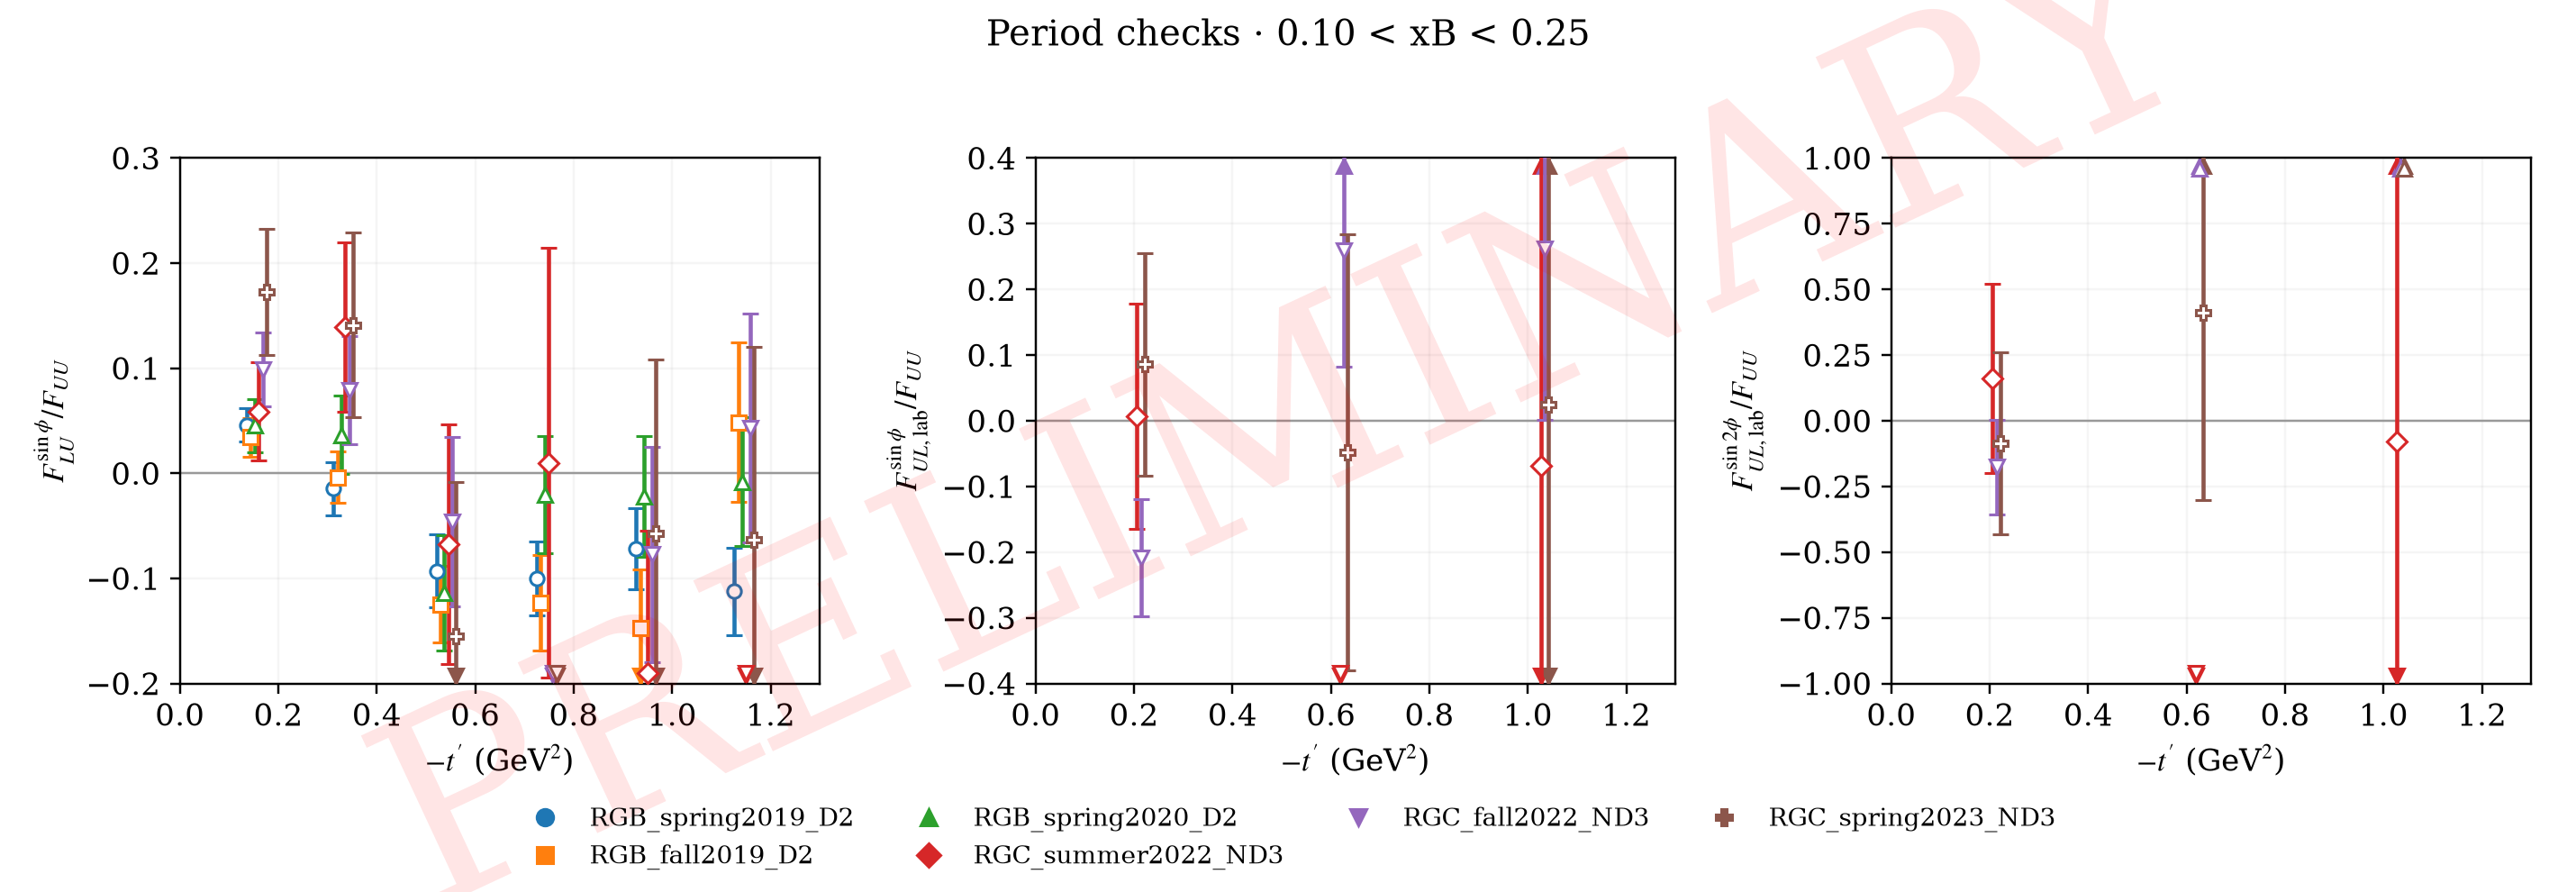
\includegraphics[width=\linewidth]{figures/results/periods_xB_bin_1.png}
\caption{Period comparison in $x_B$ interval 1. $LU$ includes the three RGB and three RGC samples; the target-spin panels show the three RGC ND$_3$ periods. Points are displaced horizontally for readability. Shared dilution uncertainties correlate target-period results.}\label{fig:release_period1}
\end{figure}
\clearpage
\begin{figure}[p]\centering
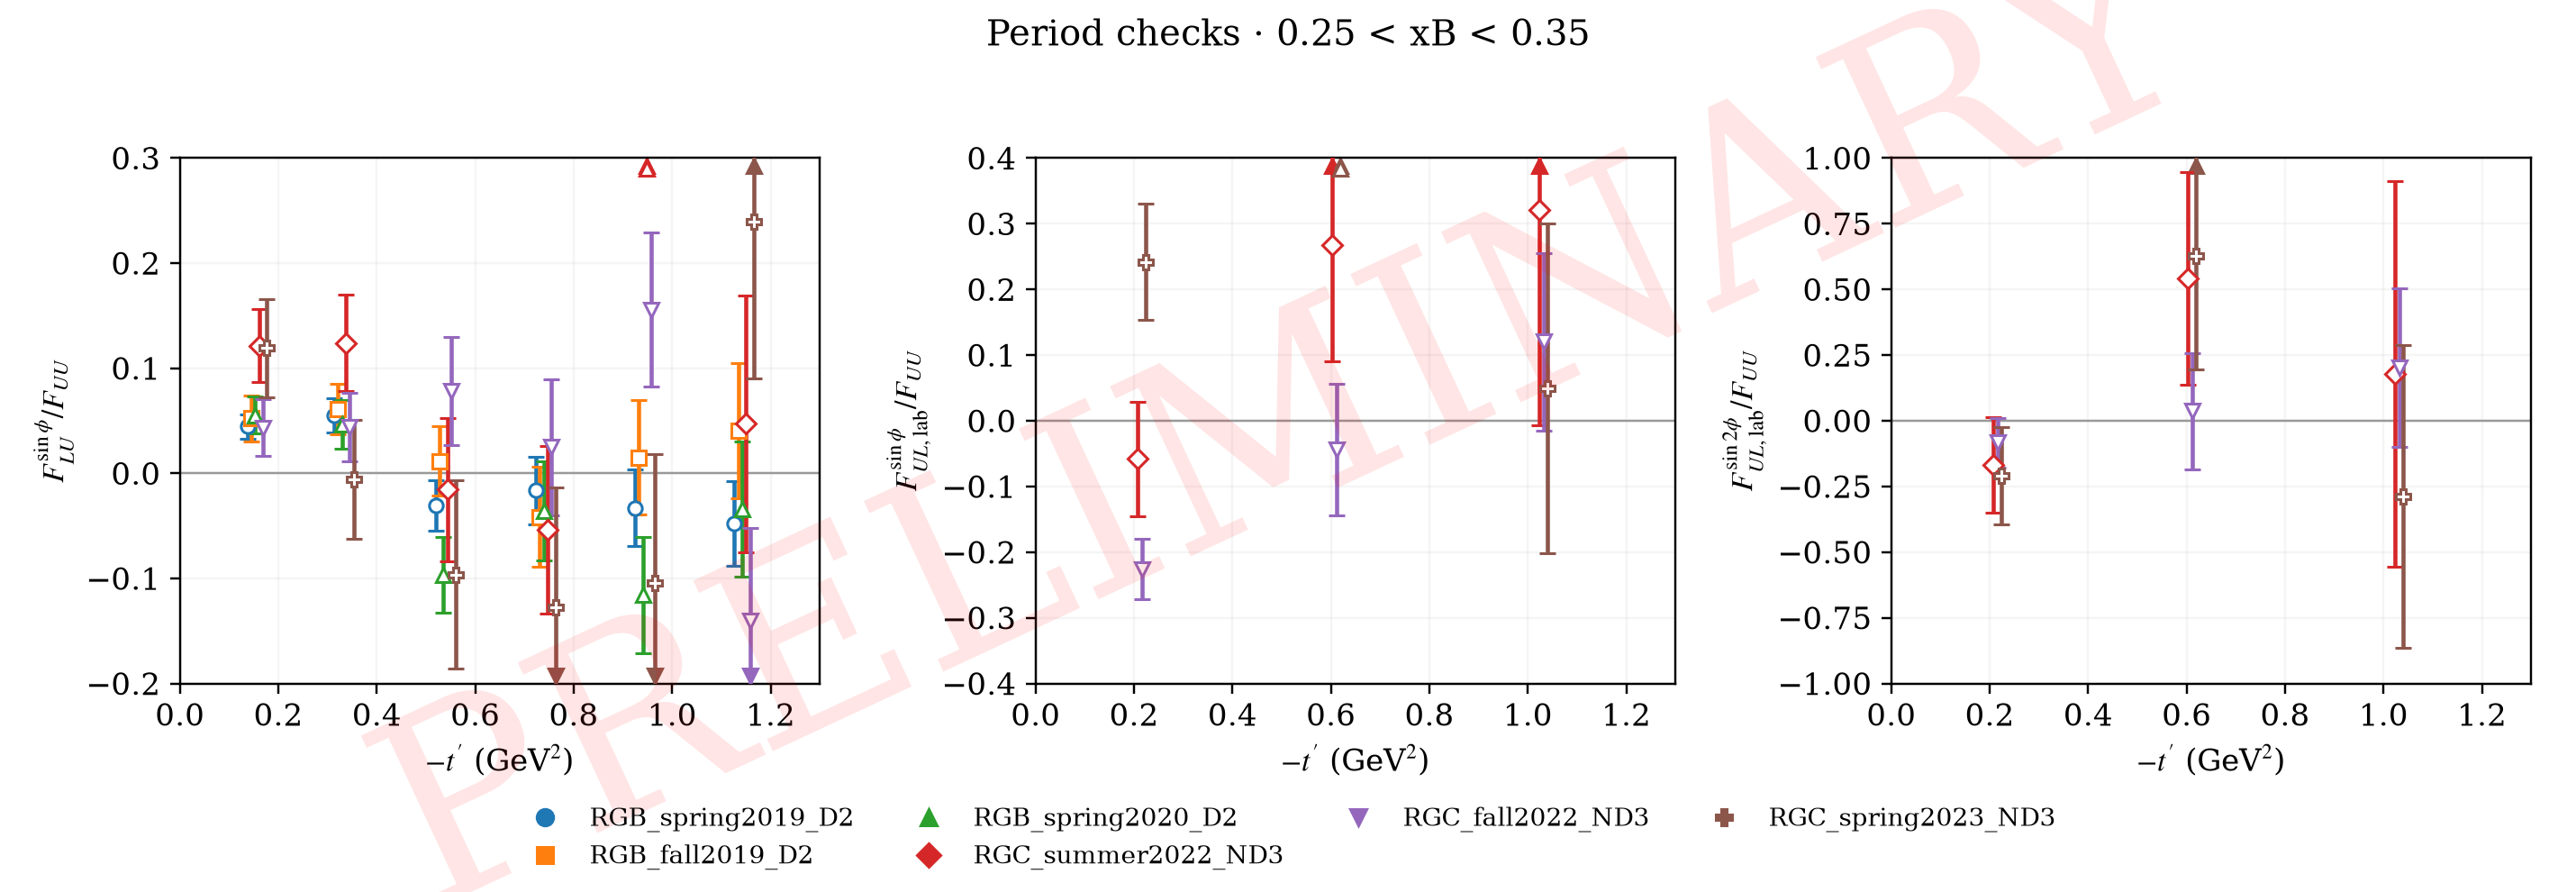
\includegraphics[width=\linewidth]{figures/results/periods_xB_bin_2.png}
\caption{Period comparison in $x_B$ interval 2. $LU$ includes the three RGB and three RGC samples; the target-spin panels show the three RGC ND$_3$ periods. Points are displaced horizontally for readability. Shared dilution uncertainties correlate target-period results.}\label{fig:release_period2}
\end{figure}
\clearpage
\begin{figure}[p]\centering
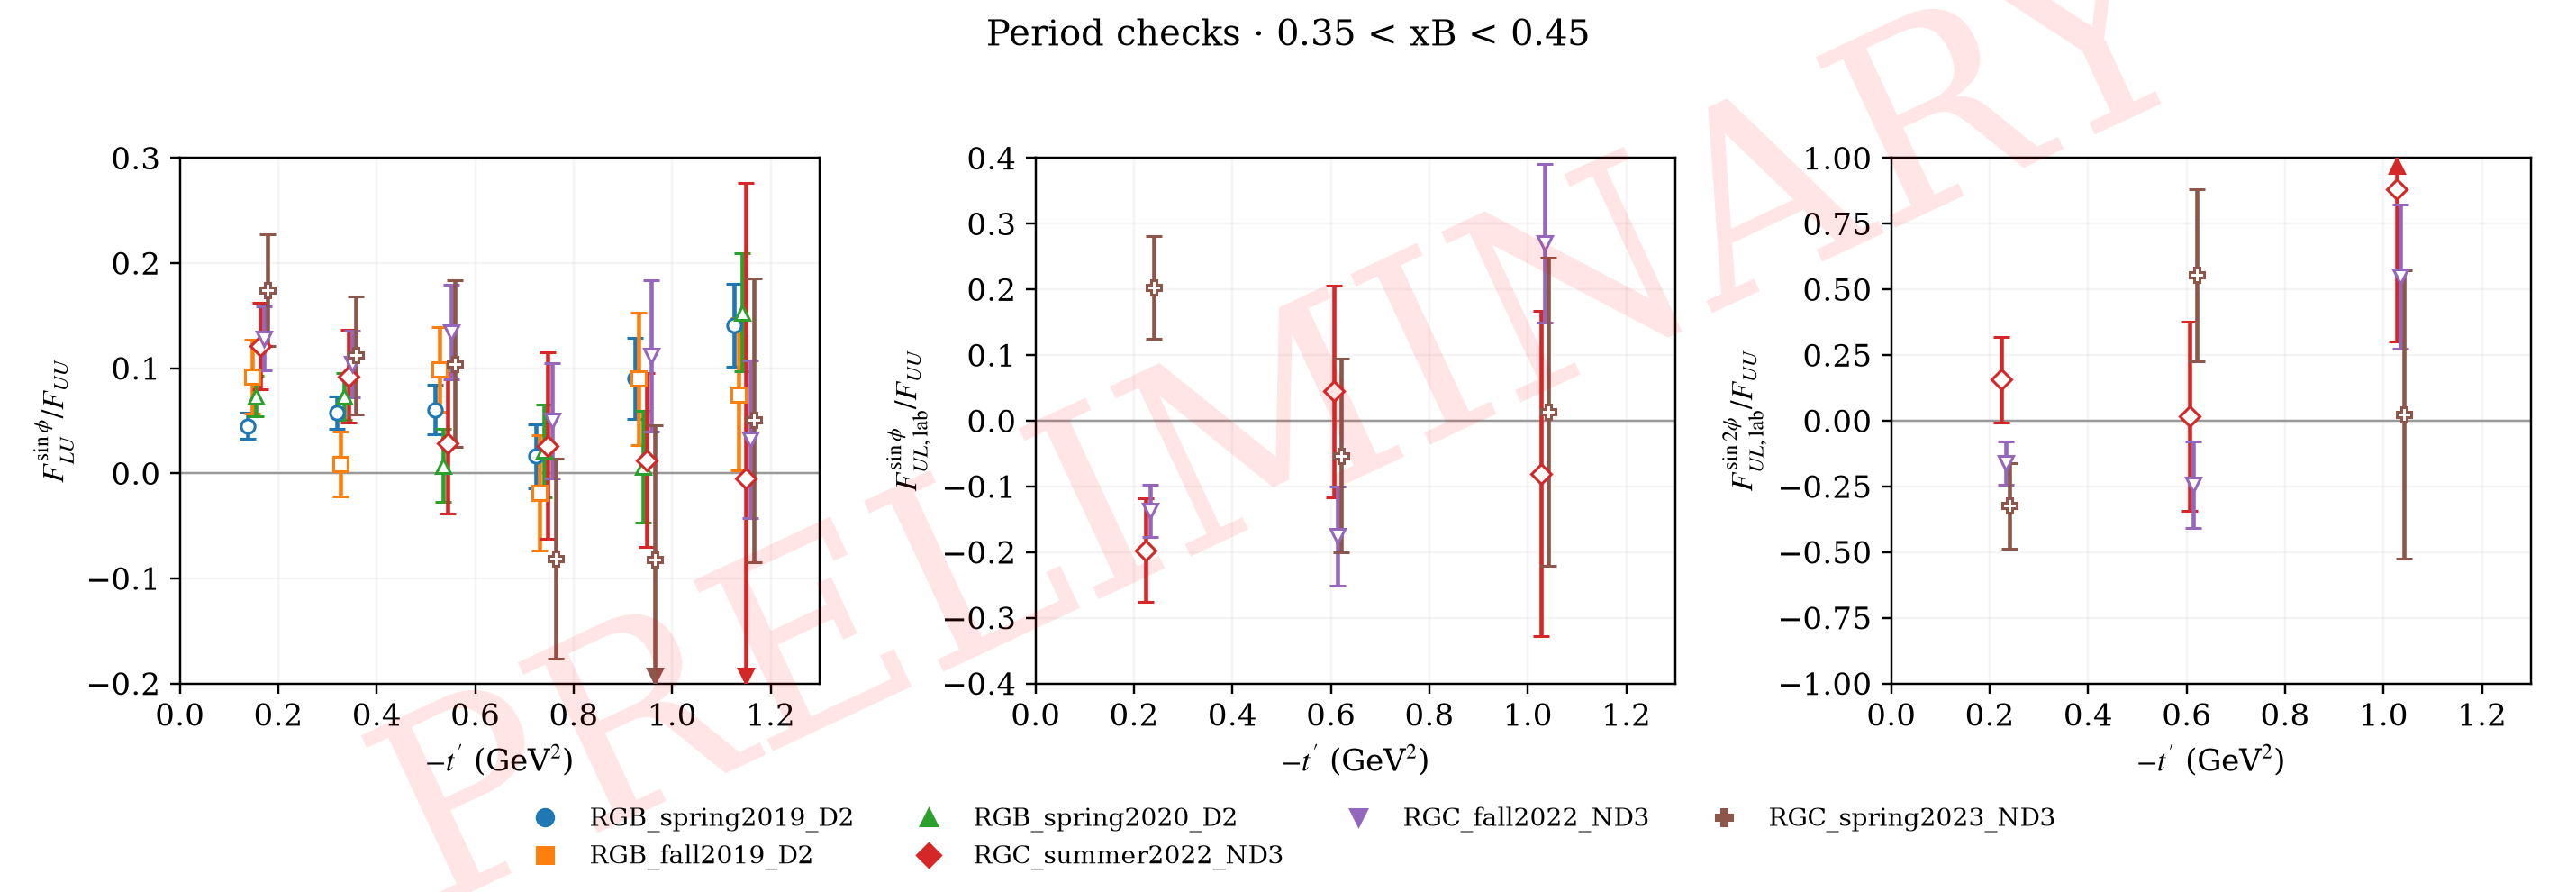
\includegraphics[width=\linewidth]{figures/results/periods_xB_bin_3.png}
\caption{Period comparison in $x_B$ interval 3. $LU$ includes the three RGB and three RGC samples; the target-spin panels show the three RGC ND$_3$ periods. Points are displaced horizontally for readability. Shared dilution uncertainties correlate target-period results.}\label{fig:release_period3}
\end{figure}
\clearpage
\begin{figure}[p]\centering
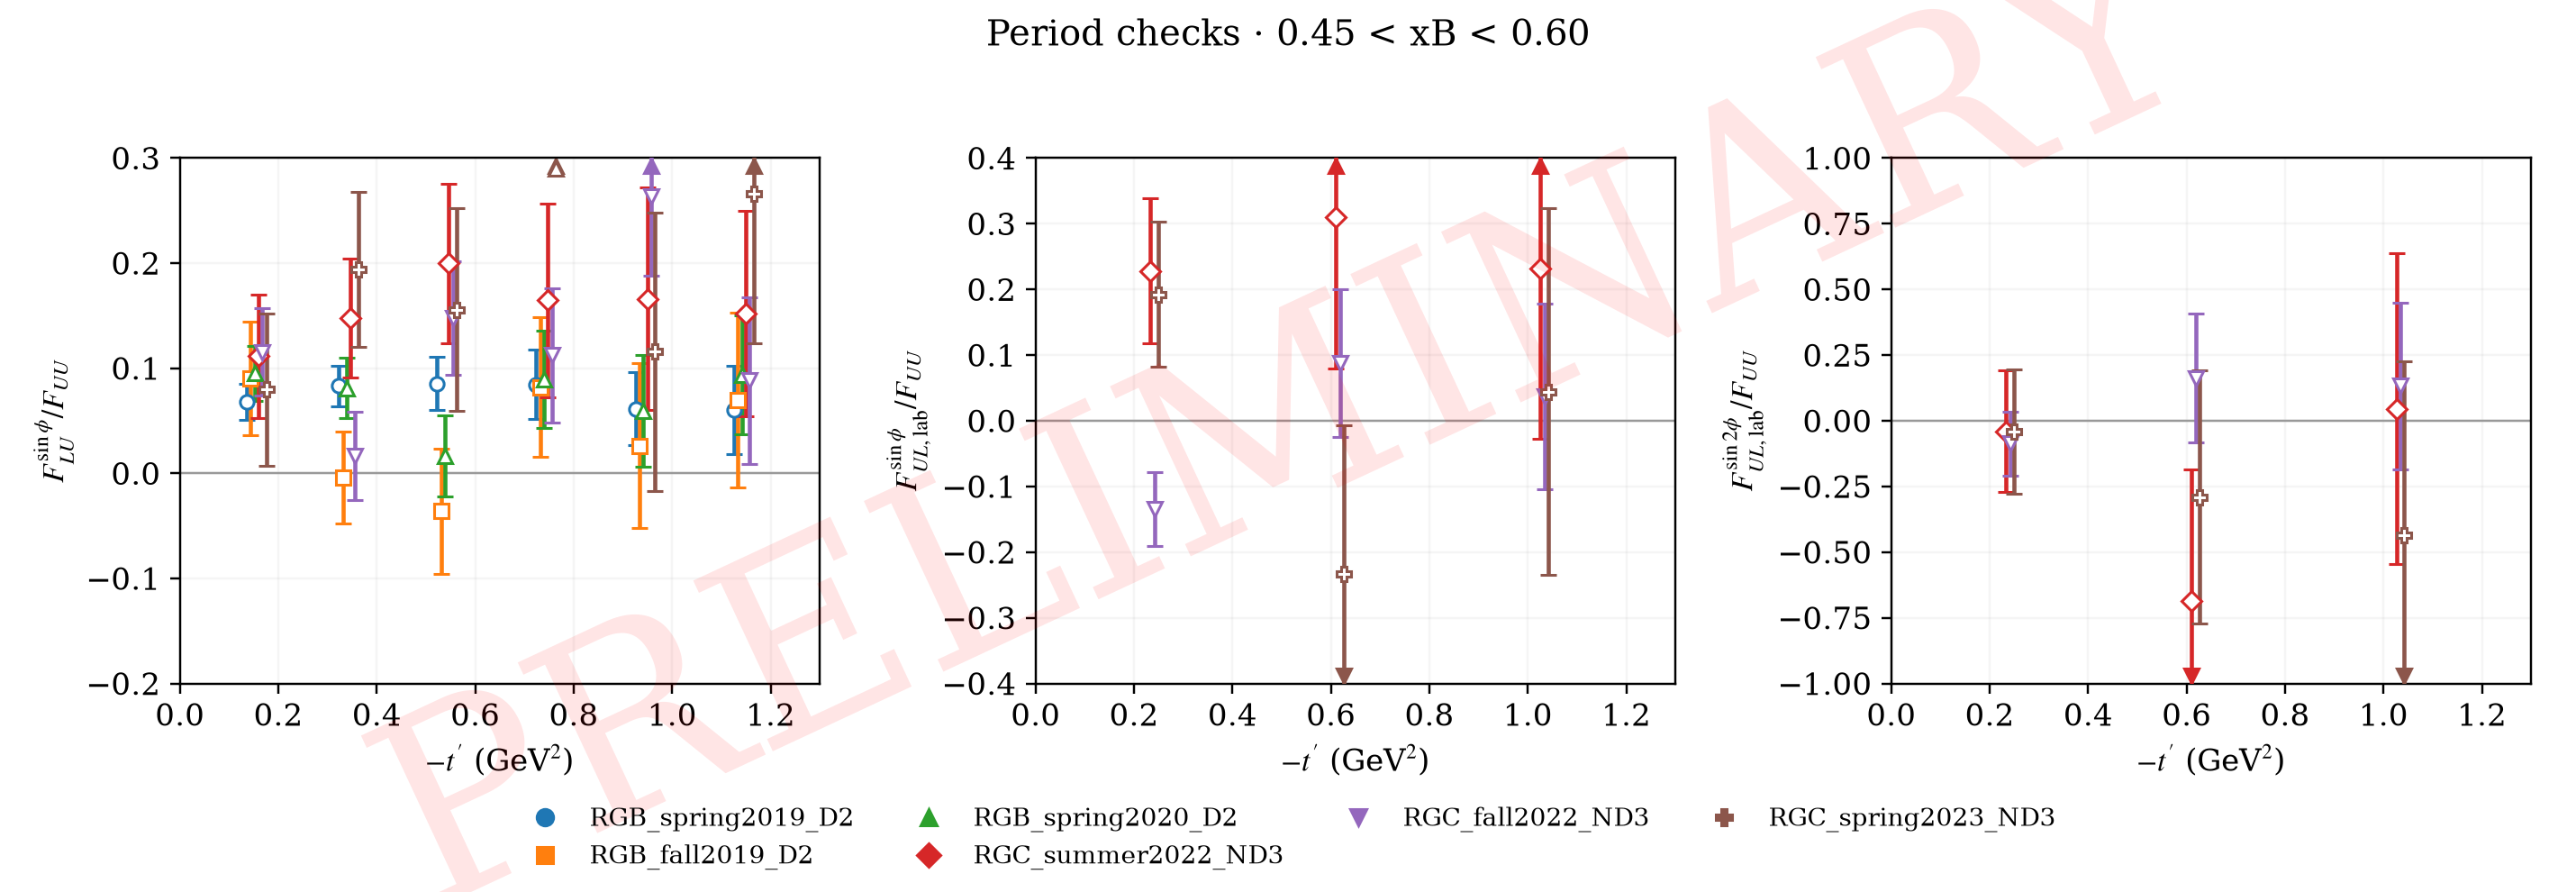
\includegraphics[width=\linewidth]{figures/results/periods_xB_bin_4.png}
\caption{Period comparison in $x_B$ interval 4. $LU$ includes the three RGB and three RGC samples; the target-spin panels show the three RGC ND$_3$ periods. Points are displaced horizontally for readability. Shared dilution uncertainties correlate target-period results.}\label{fig:release_period4}
\end{figure}
\clearpage
